\subsection{RICH detectors}

The primary aim of the \lhcb \rich system is to provide \pid separation of charged hadrons (\pion,
\kaon, and \proton).
\rich information can also be used to identify muons, although penetrating muons are identified by
the muon system.
The ability to correctly assign the correct mass hypotheses is a vital part of the \lhcb physics
program.
Since interesting $b$-hadron decays frequently result in final states with multiple hadrons,
misidentifying daughter particles would result in an increase of combinatorial background, and
a decrease in signal significance.

\begin{figure}
  \begin{center}
    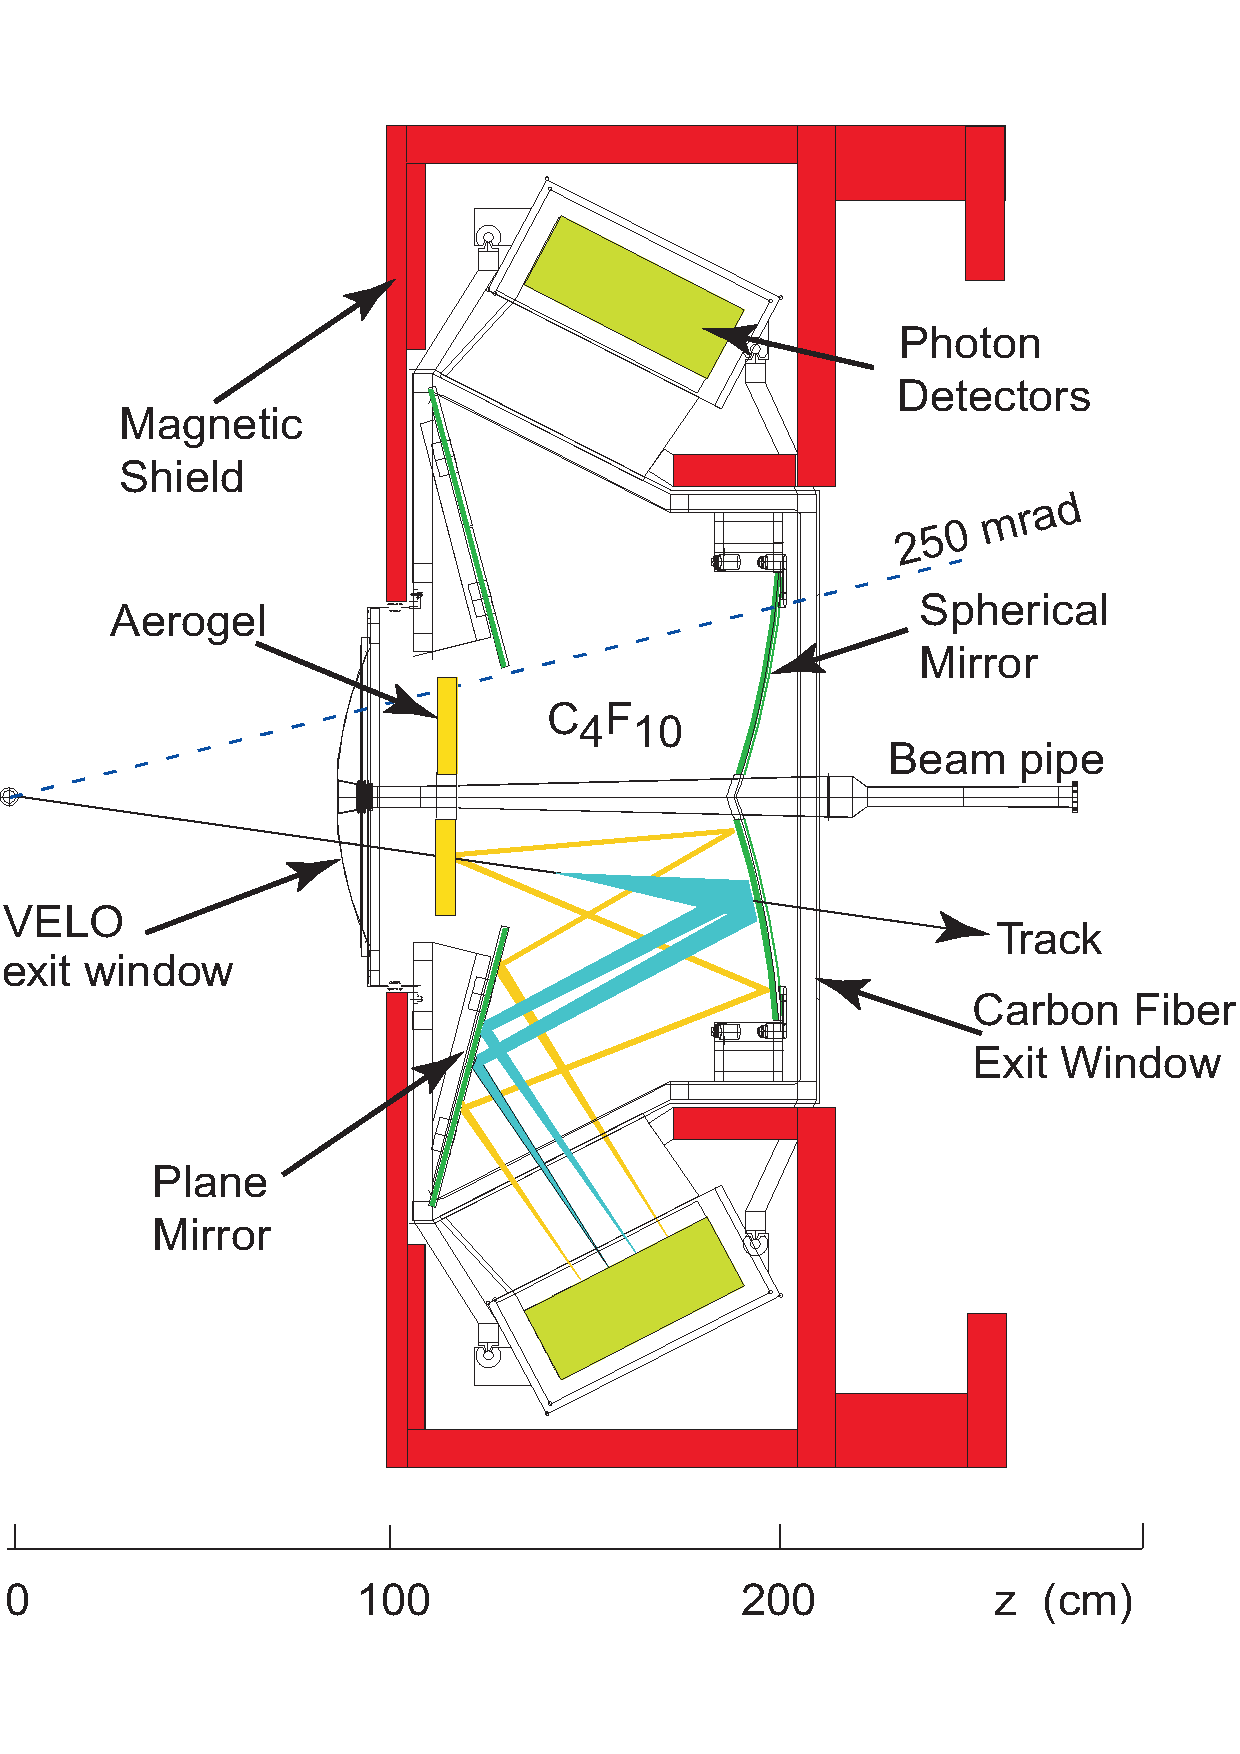
\includegraphics[height=0.43\textheight]{rich1_2d}
    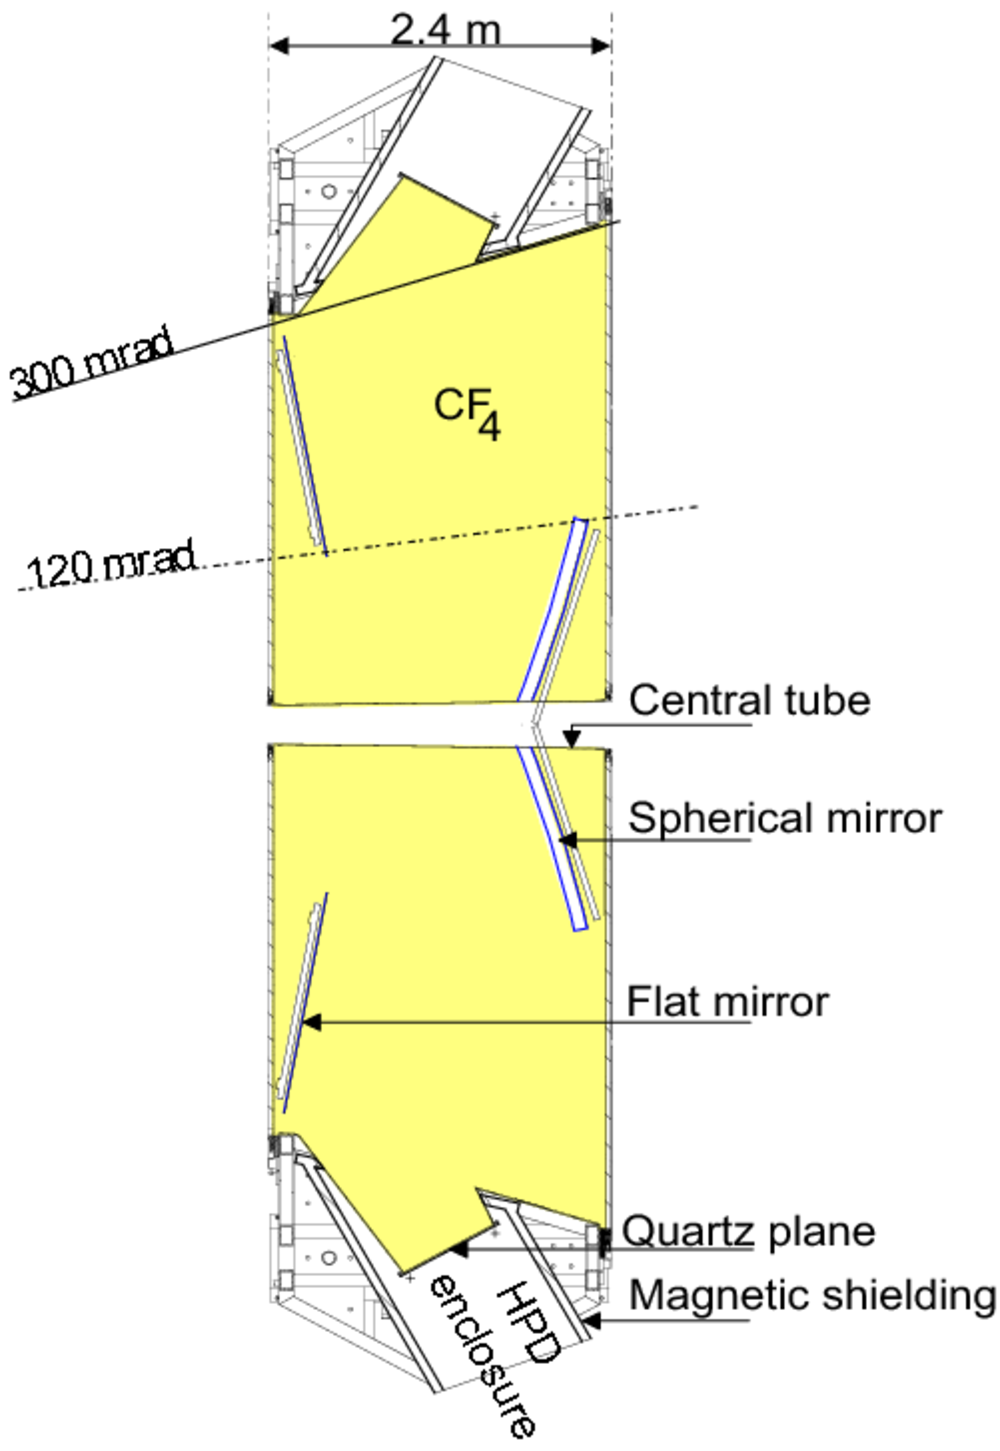
\includegraphics[height=0.43\textheight]{rich2_schematic}
    \caption[Diagmra of the LHCb RICH detectors]
    {
      Schematic diagrams of (left) \richone and (right) \richtwo, indicating the radiators,
      mirrors and HPDs.
    }
    \label{fig:lhcb:rich}
  \end{center}
\end{figure}

The principal behind the operation of the \rich system is that of Cherenkov radiation.
When a charged particle travels through a medium, with a refractive index $n$, at a greater speed
than its phase velocity, $v_p$, it decelerates by emitting a cone of light (Cherenkov radiation) in
the forward direction.
The opening angle of this light cone, $\theta_\mathrm{Ch}$, is inversely proportional to, $v_p$:
\begin{equation}
  \cos\theta_\mathrm{Ch}=\frac{c}{nv_p}.
\end{equation}
With a measurement of the particle's momentum from the tracking system and only a few possible
masses (that of the \electron, $\mu$, \pion, \kaon or \proton) likelihoods are constructed for each
track based on the ring of photons which such a particle would emit.

The \lhcb \rich system provides \pid for a wide range of momentum with the use of two \rich
detectors, containing three different radiators (aerogel and \cfourften in
\richone, and \cffour in \richtwo) between them.
Particles passing through these radiators emit a cone of photons, which are focussed using
spherical carbon fibre mirrors --- which are only $1.5\pc$ $X_0$ long --- on to an array of
\glspl{HPD}.
Figure~\ref{fig:lhcb:rich} shows schematic diagrams for \richone and \richtwo.

Different radiator materials, with different values of $n$, give the \rich system sensitivity to a
range of particle momenta.
\richone is situated immediately downstream of the \velo and covers the low momentum range,
$2<p<40\gev$, while \richtwo lies downstream of T3 and covers the range $15<p<100\gev$.
The measured quantity is that of the \gls{DLL}, where \dllxy is the difference between the
logarithm of the likelihood of the hypothesis of the particle $X$ compared to the null hypothesis of the
$Y$; where $Y$ is usually the \pion.
The variation of $\theta_\mathrm{Ch}$ on momentum for pions, kaons and protons is shown in
Fig.~\ref{fig:lhcb:pideff}.
In this way, the \lhcb detector can achieve excellent pion-kaon separation, for typical kaon
produced in a $b$-hadron decay, which has a
momentum of \approx$20\gev$, the identification rate is near $100\,\%$ and the pion misidentification
rate is a few percent as shown in Fig.~\ref{fig:lhcb:pideff}.

\begin{figure}
  \begin{center}
    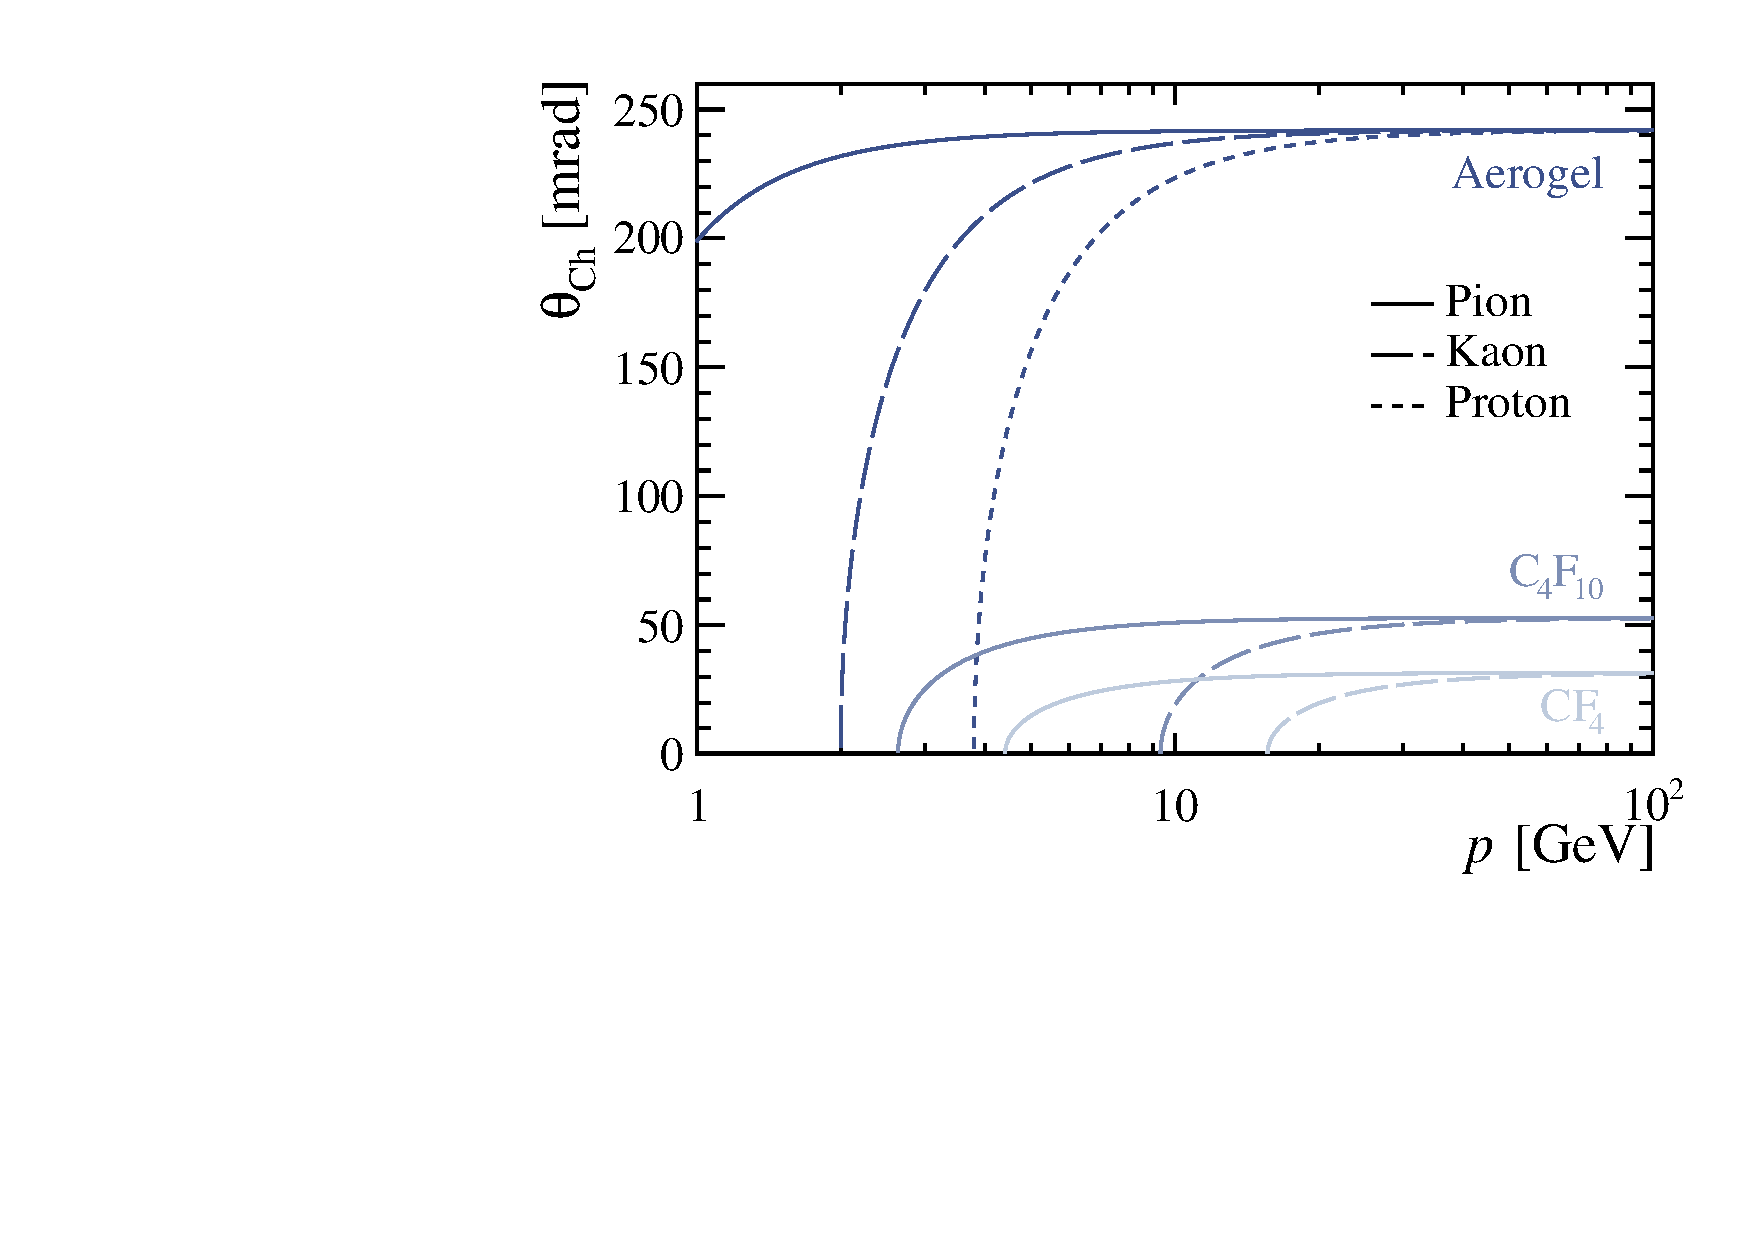
\includegraphics[height=0.2\textheight]{cherenkov_theory}
    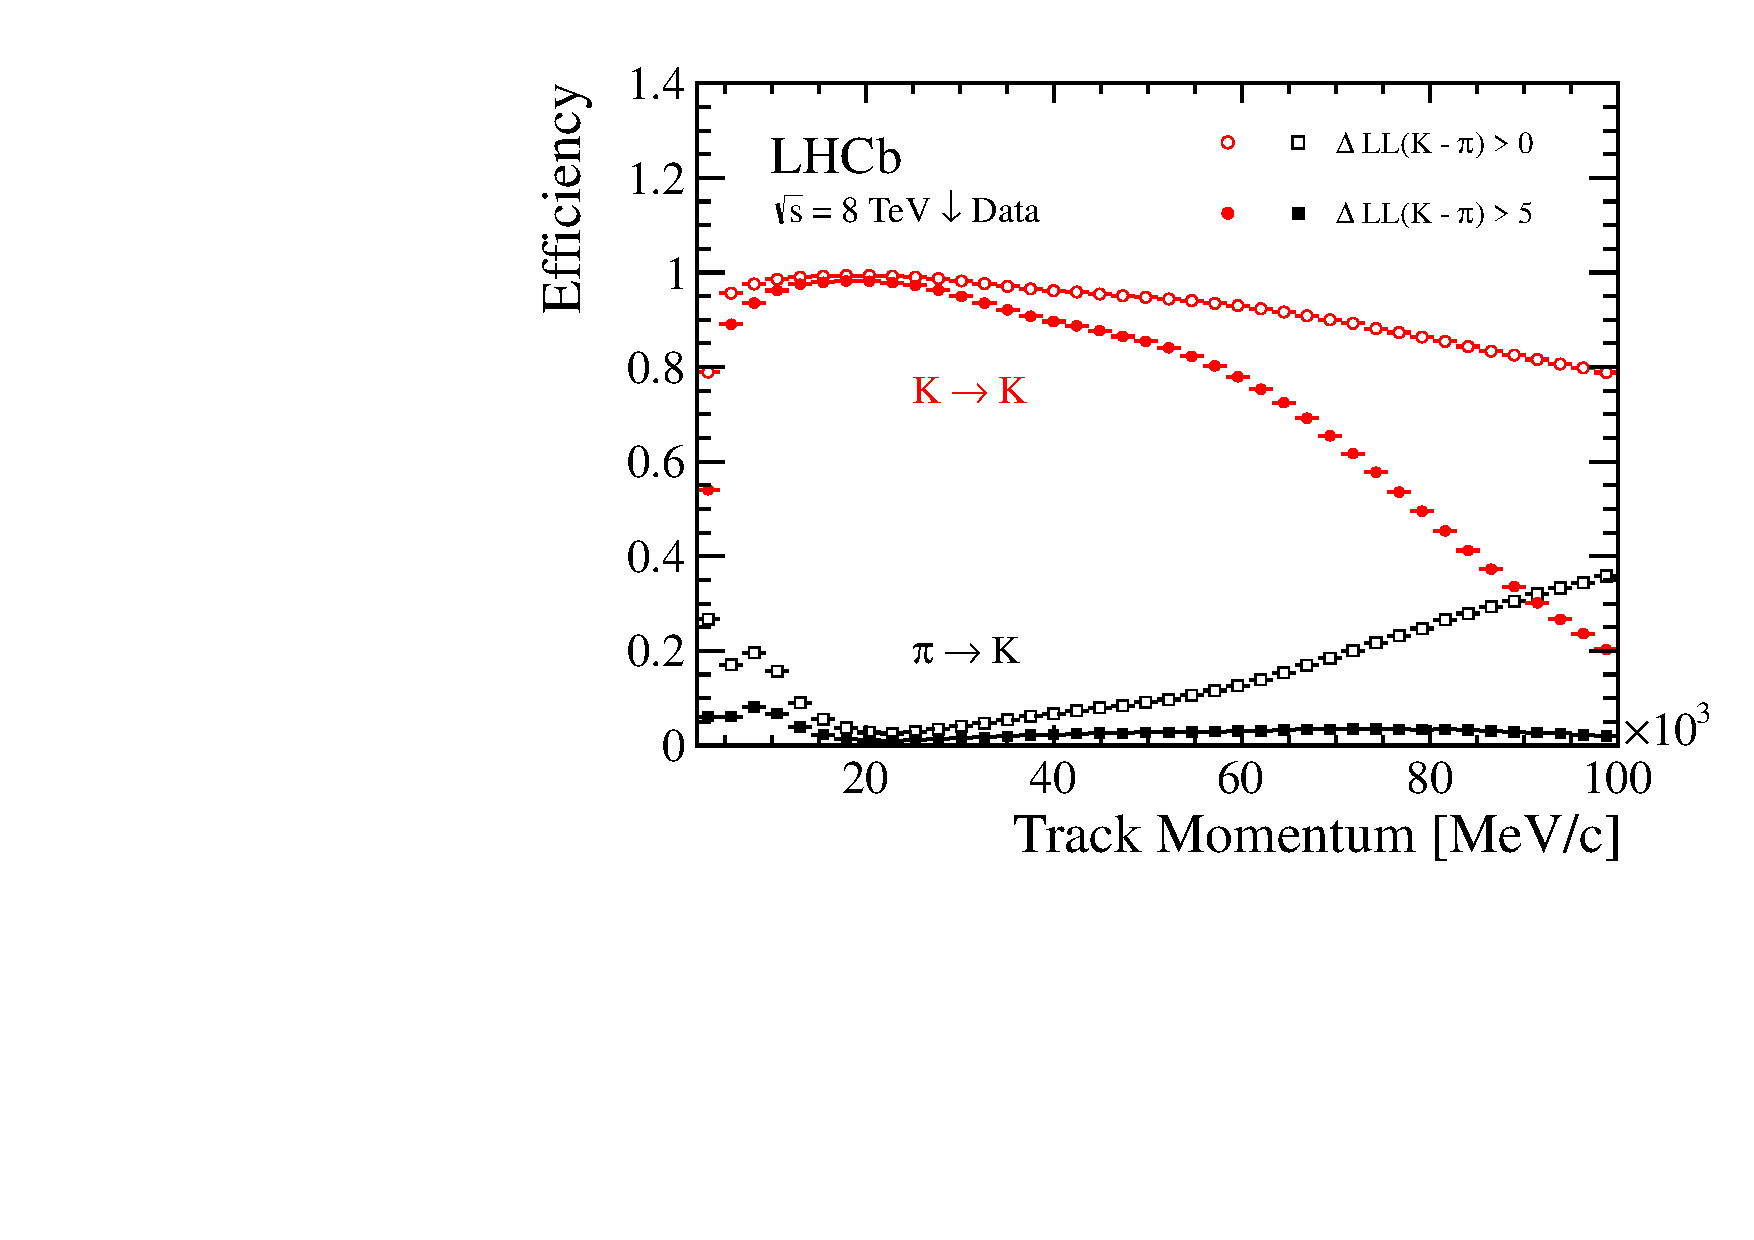
\includegraphics[height=0.2\textheight]{KPi_S20_MagDown_DLL}
  \end{center}
  \caption[Particle identification and Cherenkov angles]
  {
    Cherenkov angle as a function of momentum for pions, kaons and protons in the three different
    radiators (left), and the kaons-pion separation performance as a function of momentum, from
    Ref.~\cite{LHCb-DP-2012-003}.
  }
  \label{fig:lhcb:pideff}
\end{figure}




